%!TEX root = ../../common/main.tex

\section{Flavour physics}
\label{sec:cpv_theory:flavour_physics}

The field of flavour physics includes the description of the weak interaction of
quarks and leptons, mixing of neutral meson systems, and in general the time
evolution of those states. Inferred by the nature of the Yukawa interactions \CP
violation is possible and present in nature. In this thesis the focus is laid on
the quark sector. This introduction follows the
\Refs~\cite{Branco:1999fs,Bigi:2000yz,Agashe:2014kda}.

% ------------------------------------------------------------------------------
\subsection{The \acs{CKM} quark mixing matrix}
\label{sec:cpv_theory:flavour_physics:ckm_matrix}

To ensure local $\group{SU}{2}\otimes\group{U}{1}$ gauge invariance of the
electroweak Lagrangian while at the same time preserving renormalisability of
the theory, the mechanism of spontaneous symmetry breaking is used
\cite{set:higgs}. While the mechanism also implies new massive vector boson
fields as well as the appearance of a massive scalar particle---the Higgs
boson---the focus here will lie on the quark sector.

By introducing a complex scalar Higgs field $\phi \equiv
\left(\begin{smallmatrix} \phi ^{+} \\ \phi^{0}\end{smallmatrix}\right)$ an
$\group{SU}{2}\otimes\group{U}{1}$ invariant Yukawa Lagrangian
$\Lagrangian{Y}{}$ for the quark sector can be written as,
%
\begin{equation}\label{sec:cpv_theory:flavour_physics:ckm_matrix:yukawa_lagrangian}
  \Lagrangian{Y}{\quark} = -Y_{ij}^{\dquark\prime} \ovE{Q_{\text{L}i}} \phi \dquark_{\text{R}j}^{\prime} - Y_{ij}^{\uquark} \ovE{Q_{\text{L}i}} \phi^{\ast} \uquark_{\text{R}j} + \hc \eqcm
\end{equation}
%
with $Y_{ij}^{\quark}$ denoting the Yukawa couplings, $Q_{\text{L}i}$ being the
left-handed quark doublets, and $\quark_{\text{R}j}$ the right-handed singlets. 

By construction still being massless, the charged leptons, quarks, and the
$\Wpm$ and $\Zboson$ bosons obtain masses after the spontaneous breaking of the
symmetry and substituting the Higgs field by its \VEV
%
\begin{equation}\label{sec:cpv_theory:flavour_physics:ckm_matrix:higgs_vev}
  \langle\phi\rangle = \frac{1}{\sqrt{2}} \begin{pmatrix}
    0 \\
    v \\
  \end{pmatrix}\eqpd
\end{equation}
%
The Yukawa couplings $Y_{ij}$ are not constrained by the theory and thus are
completely arbitrary and constitute the majority of the free \SM parameters. The
coupling matrices are a priori non-diagonal in the weak interaction base, but in
general can be diagonalised by bi-unitary transformations. As a consequence of
the diagonalisation the quark fields are transformed as well into the mass
eigenstates basis allowing for flavour-changing currents through $\Wpm$ boson
exchange
%
\begin{equation}
  \frac{-g}{\sqrt{2}} \left( \uquarkbar, \cquarkbar, \tquarkbar \right)_{\text{L}} \gamma^\mu \Wp_\mu \VCKM 
  \begin{pmatrix}
    \dquark \\
    \squark \\
    \bquark \\
  \end{pmatrix}_{\text{L}} \eqcm
\end{equation}
%
with the weak charge $g$ and the transformation matrix denoted $\VCKM$
\cite{Cabibbo:1963yz,Kobayashi:1973fv}. The \CKM matrix elements $\VCKM^{ij}$
connect an up-type quark $i$ to a down-type quark $j$ with a probability
proportional to $\vert\VCKM^{ij}\vert^2$. By definition, the $3 \times 3$ \CKM
matrix is unitary, $\VCKM\VCKM^\dagger=\unity$, and complex, with $\num{18}$
free parameters. Following the unitarity conditions
%
\begin{equation}\label{sec:cpv_theory:flavour_physics:ckm_matrix:unitarity_relations}
  \sum_i V_{ij}^{\phantom{\ast}} V_{ik}^{\ast} = \delta_{jk} \eqand
  \sum_j V_{ij}^{\phantom{\ast}} V_{kj}^{\ast} = \delta_{ik} \eqcm
\end{equation}
%
and a redefinition of arbitrary quark phases, reduces the number of parameters
to three angles and one complex phase. The matrix elements are denoted as
%
\begin{equation}
  \begin{pmatrix}
    \dquark^\prime \\
    \squark^\prime \\
    \bquark^\prime \\
  \end{pmatrix}_{\text{L}}
  = 
  \begin{pmatrix}
    \Vud & \Vus & \Vub \\
    \Vcd & \Vcs & \Vcb \\
    \Vtd & \Vts & \Vtb \\
  \end{pmatrix}
  \begin{pmatrix}
    \dquark \\
    \squark \\
    \bquark \\
  \end{pmatrix}_{\text{L}}
  = \VCKM
  \begin{pmatrix}
    \dquark \\
    \squark \\
    \bquark \\
  \end{pmatrix}_{\text{L}}
\end{equation}
%
and can be expressed as a complex rotation matrix with the three angles
$\theta_{12}$, $\theta_{13}$, $\theta_{23}$ $\in {[0, \pi/2]}$ and a phase
$\delta \in {]}-\pi, \pi{]}$. With the definition of $s_{ij} \equiv \sin
\theta_{ij}$ and $c_{ij} \equiv \cos \theta_{ij}$, an exact representation
\cite{Chau:1984fp} of the \CKM matrix can be written as
%
\begin{multline}
  \VCKM = \\
  \begin{pmatrix}
    c_{12} c_{13}                                                   & s_{12} c_{13}                                                 & s_{13} \exponential{-\ii\delta} \\
    -s_{12} c_{23} - c_{12} s_{23} s_{13} \exponential{\ii\delta}   & c_{12} c_{23} - s_{12} s_{23} s_{13} \exponential{\ii\delta}  & s_{23} c_{13}                   \\
    s_{12} s_{23} - c_{12} c_{23} s_{13} \exponential{\ii\delta}    & -c_{12} s_{23} - s_{12} c_{23} s_{13} \exponential{\ii\delta} & c_{23} c_{13}                   \\
  \end{pmatrix}\eqpd
\end{multline}
%
where the phase $\delta$ is the only source of \CP violation in the \SM. A
popular approximation by Wolfenstein \cite{Wolfenstein:1983yz} takes advantage
of the measured hierarchy of the matrix elements, where the diagonal elements
are of $\order{1}$, while the off-diagonal elements follow $\vert\Vub\vert^2 \ll
\vert\Vcb\vert^2 \ll \vert\Vus\vert^2 \ll 1$ or in terms of the rotation angles
$s_{12} \ll s_{23} \ll s_{12} \ll 1$. Exploiting this hierarchy in terms of an
expansion leads to the Wolfenstein parametrisation
%
\begin{equation}  
  \VCKM = \begin{pmatrix}
    1 - \sfrac{\lambda^2}{2}         & \lambda                  & A \lambda^3 (\rho - \ii\eta) \\
    -\lambda                         & 1 - \sfrac{\lambda^2}{2} & A \lambda^2                  \\
    A \lambda^3 (1 - \rho - \ii\eta) & - A \lambda^2            & 1                            \\
  \end{pmatrix}
  + \order{\lambda^4}
\end{equation}
%
written in terms of
%
\begin{equation}
  s_{12} = \lambda, \eqspace s_{23} = A \lambda^2, \eqand s_{13}\exponential{\ii\delta} = A \lambda^3 (\rho + \ii\eta) \eqpd
\end{equation}
%
The parameters are measured in the \SM as $\lambda \approx 0.23$, $A \approx
0.81$, $\rho \approx 0.13$, and $\eta \approx 0.26$. Given the unitarity
relations in
\cref{sec:cpv_theory:flavour_physics:ckm_matrix:unitarity_relations} the six
vanishing combinations can be represented in a triangle in the complex plane.
The most prominent ${(\dquark,\bquark)}$ unitarity triangle arises from
%
\begin{equation}
  \Vud^{\phantom{\ast}}\Vub^{\ast} + \Vcd^{\phantom{\ast}}\Vcb^{\ast} + \Vtd^{\phantom{\ast}}\Vtb^{\ast} = 0 
\end{equation}
%
where normalising each side of the triangle by
$\Vcd^{\phantom{\ast}}\Vcb^{\ast}$ yields vertices at ${(0,0)}$ and ${(1,0)}$
and an apex at ${(\ovE{\rho},\ovE{\eta})}$. The area of all unitarity triangles
is of equal size and can be expressed as half of the Jarlskog invariant $J = \pm
\Im V_{ik}^{\phantom{\ast}} V_{jl}^{\phantom{\ast}} V_{il}^{\ast} V_{jk}^{\ast}$
with $i \neq j$ and $l \neq k$. It is a measure of \CP violation in the \SM and
can be determined to be $\vert J \vert = \lambda^6 A^2 \eta \approx \num{3e-5}$.

The angles and the sides of the triangle can be expressed in terms of the matrix
elements as
%
\begin{equation}
  \alpha = \arg\left(-\frac{\Vtd^{\phantom{\ast}}\Vtb^{\ast}}{\Vud^{\phantom{\ast}}\Vub^{\ast}}\right)\eqcm\eqthinspace 
  \beta =  \arg\left(-\frac{\Vcd^{\phantom{\ast}}\Vcb^{\ast}}{\Vtd^{\phantom{\ast}}\Vtb^{\ast}}\right)\eqcm\eqthinspace 
  \gamma = \arg\left(-\frac{\Vud^{\phantom{\ast}}\Vub^{\ast}}{\Vcd^{\phantom{\ast}}\Vcb^{\ast}}\right)\eqcm
\end{equation}
%
and
%
\begin{equation}
  R_t = \left| \frac{\Vtd^{\phantom{\ast}}\Vtb^{\ast}}{\Vcd^{\phantom{\ast}}\Vcb^{\ast}} \right|\eqcm\eqspace
  R_u = \left| \frac{\Vud^{\phantom{\ast}}\Vub^{\ast}}{\Vcd^{\phantom{\ast}}\Vcb^{\ast}} \right|\eqcm\eqspace
  R_c = \left| \frac{\Vcd^{\phantom{\ast}}\Vcb^{\ast}}{\Vcd^{\phantom{\ast}}\Vcb^{\ast}} \right|\eqcm
\end{equation}
%
which simplifies to
%
\begin{equation}
  R_t \exponential{-\ii\beta} + R_u \exponential{-\ii\gamma} = \unity \eqpd
\end{equation}
%
Considering various measurements of parameters of the ${(\uquark,\dquark)}$
unitarity triangle allows to constraint the apex in the
${(\ovE{\rho},\ovE{\eta})}$-plane \cite{Charles:2004jd,Bona:2006ah} as shown in
\cref{fig:cpv_theory:flavour_physics:ckm_matrix:ckm_fitter_14}.

\begin{figure}[ht]
\centering
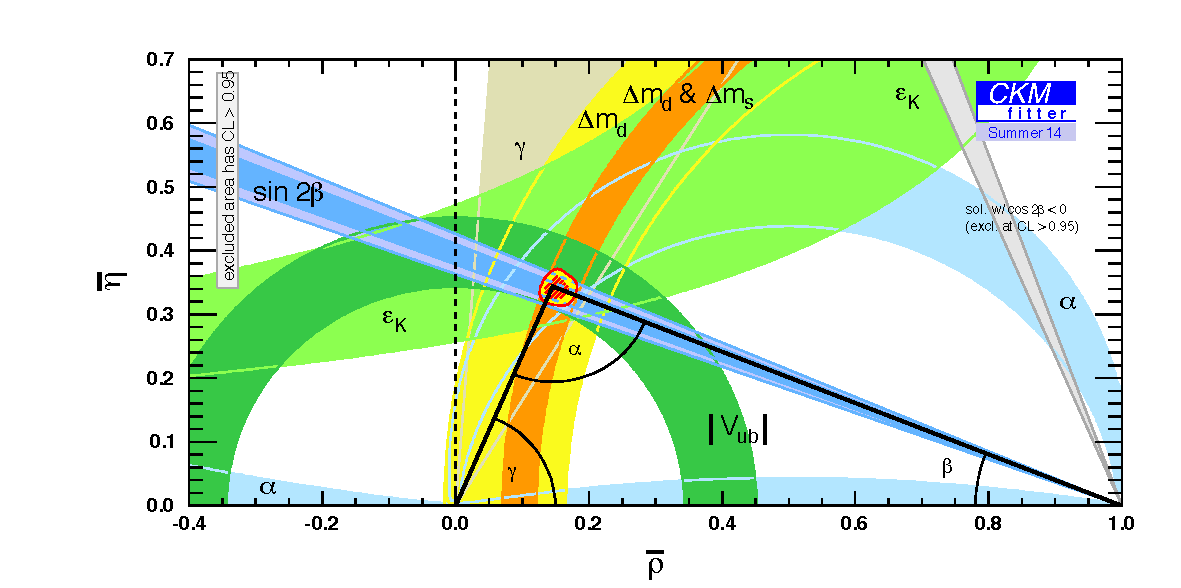
\includegraphics[width=1\textwidth]{private/content/cpv-theory/figs/ckmfitter_summer14.pdf}
\caption{Constraints on the ${(\dquark,\bquark)}$ unitarity triangle in the
${(\ovE{\rho},\ovE{\eta})}$-plane from a global fit incorporating all measured
\CKM parameters \cite{Charles:2004jd}. Regions outside the coloured areas have
$1-p > \SI{95.45}{\percent}$. The red hashed region of the global combination
corresponds to $\SI{68}{\percent}$ \acp{CL}.}
\label{fig:cpv_theory:flavour_physics:ckm_matrix:ckm_fitter_14}
\end{figure}

% ------------------------------------------------------------------------------
\subsection[
  head={\B meson decay},
  tocentry={\BHyperref meson decay}
]{\Bbfsf meson decay}
\label{sec:cpv_theory:flavour_physics:bdecays}

The decay of a meson state \Meson or its \CP conjugate state \Mesonbar into a
multi-particle final state $f$ or its \CP conjugate state $\ovE{f}$ can be
expressed by the decay amplitudes
%
\begin{equation}
  \begin{alignedat}{2}
    & A_f         = \matrixelement{f}{\Hamiltonian{}{}}{\Meson},       && \ovE{A}_f         = \matrixelement{f}{\Hamiltonian{}{}}{\Mesonbar}, \\
    & A_{\ovE{f}} = \matrixelement{\ovE{f}}{\Hamiltonian{}{}}{\Meson}, &\eqand& \ovE{A}_{\ovE{f}} = \matrixelement{\ovE{f}}{\Hamiltonian{}{}}{\Mesonbar},
  \end{alignedat}
\end{equation}
%
where \Hamiltonian{}{} is the Hamiltonian governing the weak interaction.

Under the premise of $(\CP)^2 = \unity$ the initial and final states transform under
the \CP operation as
%
\begin{equation}
  \begin{alignedat}{2}
    & \CP\ket{\Meson}    = \exponential{+\ii\zeta_{M}} \ket{\Mesonbar}, && \CP \ket{f}        = \exponential{+\ii\zeta_{f}} \ket{\ovE{f}}, \\
    & \CP\ket{\Mesonbar} = \exponential{-\ii\zeta_{M}} \ket{\Meson}   , &\eqand& \CP \ket{\ovE{f}}  = \exponential{-\ii\zeta_{f}} \ket{f},
  \end{alignedat}
\end{equation}
%
introducing phases $\zeta_M$ and $\zeta_f$. If the \CP symmetry is conserved
$\ovE{A}_{\ovE{f}} = \exponential{\ii(\zeta_f - \zeta_M)} A_f$.

% ------------------------------------------------------------------------------
\subsection[
  head={Oscillations of neutral \B mesons},
  tocentry={Oscillations of neutral \BHyperref mesons}
]{Oscillations of neutral \Bbfsf mesons}
\label{sec:cpv_theory:flavour_physics:bmixing}

To understand the oscillation of a neutral meson state $\Mesonz$ into its
$\Mesonzbar$ \CP conjugate state and vice versa, the time evolution of the meson
states has to be studied. Given a pure \Mesonz or \Mesonzbar initial state at
$t=0$, it will evolve in time acquiring components that describe all possible final states $f_1, f_2, \dots$,
%
\begin{equation}
  \ket{\Psi(t)} = \psi_1(t) \ket{\Mesonz} + \psi_2(t) \ket{\Mesonzbar} + c_1(t) \ket{f_1} + c_2(t) \ket{f_2} + \dots \eqpd
\end{equation}
%
As only the parameters $\psi_1(t)$ and $\psi_2(t)$ are of interest, this time
evolution can be described by a Schrödinger-like equation,
%
\begin{equation}
  i \frac{\dif}{\dif t} 
  \begin{pmatrix}
    \psi_1 \\
    \psi_2
  \end{pmatrix}
  =
  \Hamiltonian{}{}
  \begin{pmatrix}
    \psi_1 \\
    \psi_2
  \end{pmatrix}
  =
  \begin{pmatrix}
    m_{11} - \frac{\ii}{2} \mathit{\Gamma}_{11}    & m_{12} - \frac{\ii}{2} \mathit{\Gamma}_{12} \\
    m_{21} - \frac{\ii}{2} \mathit{\Gamma}_{21}    & m_{22} - \frac{\ii}{2} \mathit{\Gamma}_{22} \\
  \end{pmatrix}
  \begin{pmatrix}
    \psi_1 \\
    \psi_2
  \end{pmatrix}\eqcm
\end{equation}
%
following the Weisskopf-Wigner approximation
\cite{Weisskopf:1930au,Weisskopf:1930ps} with two Hermitian $2\times2$ matrices
$M$ and $\mathit{\Gamma}$, where the Hamiltonian
%
\begin{equation}
  \Hamiltonian{}{} = M - \frac{\ii}{2} \mathit{\Gamma}
\end{equation}
%
is not Hermitian, as otherwise the meson states would just oscillate without
decaying.

Assuming \CPT invariance, $m_{11} = m_{22} = m$, $m_{21} = m_{12}^{\ast}$,
$\mathit{\Gamma}_{11} = \mathit{\Gamma}_{22} = \mathit{\Gamma}$, and
$\mathit{\Gamma}_{21} = \mathit{\Gamma}_{12}^{\ast}$. Diagonalising the
Hamiltonian yields eigenstates with well-defined masses
%
\begin{equation}\label{eq:cpv_theory:flavour_physics:bmixing:mass_eigenstates}
  \begin{split}
    \ket{\Mesonz_L} &= p \ket{\Mesonz} + q \ket{\Mesonzbar}\eqcm\eqand \\
    \ket{\Mesonz_H} &= p \ket{\Mesonz} - q \ket{\Mesonzbar}\eqcm
  \end{split}
\end{equation}
%
with $\abs{q}^2 + \abs{p}^2 = 1$, where $\Meson_L$ marks the light and
$\Meson_H$ the heavy eigenstate. The correspondent eigenvalues are
%
\begin{equation}
  \begin{split}
    \mu_H &= m_H - \frac{\ii}{2} \mathit{\Gamma}_H\eqcm\eqand \\
    \mu_L &= m_L - \frac{\ii}{2} \mathit{\Gamma}_L\eqpd
  \end{split}
\end{equation}
%
with the definitions of the average mass and decay width
%
\begin{equation}
  m = \frac{m_H + m_L}{2} \eqcm \eqand \mathit{\Gamma} = \frac{\mathit{\Gamma}_H + \mathit{\Gamma}_L}{2}\eqcm
\end{equation}
%
and the mass and decay width differences
%
\begin{equation}
  \DM = m_H - m_L \eqcm \eqand \DG = \mathit{\Gamma}_H - \mathit{\Gamma}_L\eqpd
\end{equation}
%
The mass difference $\DM$ of the two mass eigenstates is by definition positive
while the sign of $\DG$ has to be determined experimentally.

% ------------------------------------------------------------------------------
\subsection{Time evolution of meson states}
\label{sec:cpv_theory:flavour_physics:time_evolution}

After an outline of the decay and the oscillation of \Bmesons and the \CKM
mechanism in the \SM the time evolution and differential decay rates are defined
in the following. The time evolution of a physical state produced as $t=0$
either as a pure $\ket{\Mesonz}$ or $\ket{\Mesonzbar}$ state is now described by
%
\begin{equation}
  \begin{split}
    \ket{\Mesonz_{\text{phys}} (t)}    &= g_{+}(t) \ket{\Mesonz}    - \frac{q}{p} g_{-}(t) \ket{\Mesonzbar} \eqcm \eqand\\
    \ket{\Mesonzbar_{\text{phys}} (t)} &= g_{+}(t) \ket{\Mesonzbar} - \frac{p}{q} g_{-}(t) \ket{\Mesonz}    \eqcm
  \end{split}
\end{equation}
%
where the coefficients $g_{\pm}$ are defined as
%
\begin{equation}
  g_{\pm}(t) \equiv 
  \frac{1}{2} \left[
    \exponential{-\ii \mu_H t} \pm \exponential{-\ii \mu_L t}
  \right]
  =
  \frac{1}{2} \left[
    \exponential{-\ii m_H t} \exponential{-\frac{1}{2} \mathit{\Gamma}_H t} \pm \exponential{-\ii m_L t} \exponential{-\frac{1}{2} \mathit{\Gamma}_L t}
  \right]\eqpd
\end{equation}
%
The decay rate of a meson produced at $t=0$ to a final state $f$ at time $t$
is given by the matrix element
%
\begin{equation}
  \Gamma \left(\Meson(t)\to f\right)= \bigl\vert \matrixelement{f}{T}{\Meson} \bigr\vert^2 \eqcm
\end{equation}
%
which yields the four differential decay rates  
%
\begin{equation}\label{eq:cpv_theory:flavour_physics:time_evolution:differential_decay_rates}
  \begin{split}
    \frac{\Gamma \bigl(\Meson   (t) \to       f \bigr)}{\exponential{-\Gamma t}} &= 
      \frac{1}{2} \abs{A_f}^2 \left( 1 + \abs{\lambda_f}^2 \right) \\
        \Biggl[ \cosh\Bigl(\frac{\DG t}{2}&\Bigr) + D_f \sinh\left(\frac{\DG t}{2}\right) + C_f \cos(\DM t) - S_f \sin(\DM t) \Biggr]\eqcm \\
    \frac{\Gamma \bigl(\Meson   (t) \to \ovE{f} \bigr)}{\exponential{-\Gamma t}} &= 
      \frac{1}{2} \abs{\ovE{A}_{\ovE{f}}}^2 \left( 1 + \abs{\ovE{\lambda}_{\ovE{f}}}^2 \right) \abs{\frac{q}{p}}^2 \\
        \Biggl[ \cosh\Bigl(\frac{\DG t}{2}&\Bigr) + D_{\ovE{f}} \sinh\left(\frac{\DG t}{2}\right) + C_{\ovE{f}} \cos(\DM t) - S_{\ovE{f}} \sin(\DM t) \Biggr]\eqcm \\
    \frac{\Gamma \bigl(\Mesonbar(t) \to       f \bigr)}{\exponential{-\Gamma t}} &= 
      \frac{1}{2} \abs{A_f}^2 \left( 1 + \abs{\lambda_f}^2 \right) \abs{\frac{p}{q}}^2 \\
        \Biggl[ \cosh\Bigl(\frac{\DG t}{2}&\Bigr) + D_f \sinh\left(\frac{\DG t}{2}\right) - C_f \cos(\DM t) + S_f \sin(\DM t) \Biggr]\eqcm \\
    \frac{\Gamma \bigl(\Mesonbar(t) \to \ovE{f} \bigr)}{\exponential{-\Gamma t}} &= 
      \frac{1}{2} \abs{\ovE{A}_{\ovE{f}}}^2 \left( 1 + \abs{\ovE{\lambda}_{\ovE{f}}}^2 \right) \\
        \Biggl[ \cosh\Bigl(\frac{\DG t}{2}&\Bigr) + D_{\ovE{f}} \sinh\left(\frac{\DG t}{2}\right) - C_{\ovE{f}} \cos(\DM t) + S_{\ovE{f}} \sin(\DM t) \Biggr]\eqcm \\
  \end{split}
\end{equation}
%
where the definitions
%
\begin{equation}\label{eq:cpv_theory:flavour_physics:time_evolution:lambdaf}
  \lambda_f               \equiv \frac{1}{\ovE{\lambda}_f}   = \frac{q}{p} \frac{\ovE{A}_f}{A_f}                 \eqcm \eqand 
  \ovE{\lambda}_{\ovE{f}} \equiv \frac{1}{\lambda_{\ovE{f}}} = \frac{p}{q} \frac{A_{\ovE{f}}}{\ovE{A}_{\ovE{f}}}
\end{equation}
%
are used.

The \CP coefficients $D_i$, $C_i$, and $S_i$ have to satisfy $D_i^2 + C_i^2 +
S_i^2 = 1$ and are defined as
%
\begin{equation}\label{eq:cpv_theory:flavour_physics:time_evolution:cp_coefficients}
  \begin{alignedat}{2}
    &D_f = \frac{2 \Re \lambda_f}      {1+\abs{\lambda_f}^2},   \eqspace 
    &C_f = \frac{1 - \abs{\lambda_f}^2}{1 + \abs{\lambda_f}^2}, \eqspace 
    &S_f = \frac{2 \Im \lambda_f}      {1+\abs{\lambda_f}^2}    \eqcm \eqand \\
    &D_{\ovE{f}} = \frac{2 \Re \ovE{\lambda}_{\ovE{f}}}      {1+\abs{\ovE{\lambda}_{\ovE{f}}}^2},   \eqspace 
    &C_{\ovE{f}} = \frac{1 - \abs{\ovE{\lambda}_{\ovE{f}}}^2}{1 + \abs{\ovE{\lambda}_{\ovE{f}}}^2}, \eqspace 
    &S_{\ovE{f}} = \frac{2 \Im \ovE{\lambda}_{\ovE{f}}}      {1+\abs{\ovE{\lambda}_{\ovE{f}}}^2}    \eqpd \\
  \end{alignedat}
\end{equation}
%

\subsection[Classification of \CP violating effects]{Classification of \CPbfsf violating effects}
\label{sec:cpv_theory:flavour_physics:cpv_classification}

While a single phase in the \CKM quark mixing matrix is the only source of \CP
violation in the \SM, \CP violation appears in different manifestations.

\subsubsection[Direct \CP violation]{Direct \CPbfsf violation}
\label{sec:cpv_theory:flavour_physics:cpv_classification:direct}

\CP violation in the decay---also called direct \CP violation---occurs if the
decay amplitudes of a meson into a final state differ from the \CP conjugate
decay
%
\begin{equation}
  \frac{\abs{\ovE{A}_{\ovE{f}}}}{\abs{A_f}} \neq 1 \eqpd
\end{equation}
%
This is the only possible source of \CP violation in charged mesons and all
baryons. As \CP violation in the decay is expressed by the decay amplitudes, the
strength can be estimated by studying the involved \CKM matrix elements. In the
decay of \BdToJpsiKS the matrix elements $\Vcs \approx 1$ and $\Vcb
\approx A\lambda^2$ are most relevant, thus no complex phase is present up to
the order of $\lambda^2$ and no direct \CP violation is expected.

\subsubsection[\CP violation in mixing]{\CPbfsf violation in mixing}
\label{sec:cpv_theory:flavour_physics:cpv_classification:mixing}

The second class of \CP violation is denoted \CP violation in the mixing. It
occurs if
%
\begin{equation}
  \abs{\frac{q}{p}} \neq 1 \eqpd
\end{equation}
%
A potential \CP violation in the mixing of $\BdBdbar$ mesons was studied at the
\BFactories by measuring $\absinline{\sfrac{q}{p}} - 1$. The final \BFactory
average shows no significant deviation from zero: $\absinline{\sfrac{q}{p}} - 1
= \num{0.3 +- 2.8 e-3}$ \cite{Bevan:2014iga}. The recent measurement of the
semileptonic \CP asymmetry $a_{\text{sl}}^{\dquark}$ by the \acs*{LHCb}
collaboration confirms the quoted result. The measurement yields
$a_{\text{sl}}^{\dquark} = \bigl(-0.02 \pm 0.19 \statp \pm 0.30 \systp
\bigr)\si{\percent}$ \cite{Aaij:2014nxa} that can be expressed as
%
\begin{equation}
  \abs{\frac{q}{p}} - 1 = \bigl(0.1 \pm 0.9 \statp \pm 1.4 \systp \bigr) \times 10^{-3} \eqcm
\end{equation}
%
by employing the identity relation
%
\begin{equation}
  \abs{\frac{q}{p}} \equiv \left(\frac{1 - a_{\text{sl}}^{\dquark}}{1 + a_{\text{sl}}^{\dquark}}\right)^{\frac{1}{4}} \eqpd
\end{equation}
%

\subsubsection[\CP violation in the interference]{\CPbfsf violation in the interference}
\label{sec:cpv_theory:flavour_physics:cpv_classification:interference}

The third kind of \CP violation only occurs in decays where both \CP conjugate
initial states \Mesonz and \Mesonzbar decay into a common final state $f$. Then
an interference between a decay without mixing, $\decay{\Mesonz}{f}$, and a
decay with mixing, $\decay{\Mesonz}{\decay{\Mesonzbar}{f}}$, can lead to \CP
violation in the interference between both amplitudes of:
%
\begin{equation}
  \Im \lambda_f \neq 0 \eqpd
\end{equation}
%
As can be seen in the definition of $\lambda_f$ given in
\cref{eq:cpv_theory:flavour_physics:time_evolution:lambdaf} this type of \CP
violation even occurs if no direct \CP violation or \CP violation in mixing is
present.
